\documentclass[11pt,a4paper]{article}

\usepackage[utf8]{inputenc}
\usepackage[T1]{fontenc}
\usepackage[margin=2.4cm]{geometry}
\usepackage{amsmath,amssymb}
\usepackage{amsthm}
\theoremstyle{definition}
\newtheorem{definition}{Definition}
\usepackage{booktabs}
\usepackage{array}
\usepackage{enumitem}
\usepackage{xcolor}
\usepackage{graphicx}
\graphicspath{{images/}}
\usepackage{tikz}
\usetikzlibrary{arrows.meta,positioning,fit,backgrounds,calc}
\usepackage{hyperref}
\hypersetup{colorlinks=true,linkcolor=black,citecolor=black,urlcolor=blue!50!black}

\setlength{\parskip}{5pt}
\setlength{\parindent}{0pt}

\title{Experimentation protocol (working draft)\\[2pt]
\large Unsupervised structural clustering of the eukaryotic virome}
\author{Pascal Nardi --- M2 internship}
\date{\today}

\begin{document}
\maketitle

\tableofcontents
\vspace{4pt}
\hrule

\section{General idea}

Viral proteins change in sequence much faster than they change in shape. Because
of that, the usual sequence-based homology searches miss real relationships that
are still visible at the level of the 3D fold. The idea behind DeltaFold is to
learn, without labels, an embedding space where two viral proteins end up close
together when they share a fold, so that clustering the embeddings recovers known
protein families and possibly suggests structural links that sequence methods
cannot find.

So the biological question I would like the method to be able to answer is
whether an unsupervised structural encoder can recover viral protein families,
and whether it can connect families that have diverged in sequence but are still
structurally related. The methodological question I would like your opinion on is
whether the setup below is enough to tell apart real structural learning from the
model just exploiting easy shortcuts or collapsing its representation.

\section{Dataset}

\subsection{Source}

I use the predicted structural proteome of the eukaryotic virome from Nomburg et
al.~\cite{nomburg2024}. The release has 67,715 predicted protein structures
across 4,463 eukaryotic viral species. The structures are organised by family on
disk, which gives me weak family labels. I only use those labels to evaluate the
model, never during training.

The dataset is developed further in later sections; the featurization of each
structure and the train/validation split are deferred to
Section~\ref{sec:featurization}, after the combinatorial-complex formalism they
rely on.

\section{Topological deep learning: from CNNs to CCNNs}

This section gives the theoretical background that the architecture rests on. The
goal is to explain why a topological model is a natural choice for protein
structure, by following the line CNN $\to$ GNN $\to$ CCNN in which each step lifts
a limitation of the previous one, and to make precise the notion of equivariance
that organises this progression.

\subsection{Equivariance and invariance}

Let a group $G$ act on an input space $\mathcal{X}$ and on an output space
$\mathcal{Y}$. A map $f:\mathcal{X}\to\mathcal{Y}$ is $G$-equivariant if
\[
 f(g\cdot x)=g\cdot f(x)\qquad\text{for all }g\in G,\ x\in\mathcal{X},
\]
and $G$-invariant if $f(g\cdot x)=f(x)$ for all $g,x$, the special case where $G$
acts trivially on the output. Equivariance encodes a symmetry that the problem is
known to have, so that the model does not need to learn it from data. The three
families below are each defined by the symmetry group they respect, and each
enlarges the domain on which the model can act.

\subsection{Convolutional networks: grids and translation}

A convolutional network acts on data supported on a regular grid (image pixels,
audio samples). A convolutional layer slides one small filter across all
positions; sharing the filter makes the layer equivariant to the translation
group, that is, shifting the input shifts the output by the same amount. Weight
sharing also gives locality and a parameter count independent of the input size.
The limitation is that a grid is a rigid domain with a fixed neighbourhood and a
global coordinate system, so CNNs do not apply to data whose elements have no
canonical ordering or position, such as the residues of a protein whose contacts
are irregular.

\subsection{Graph neural networks: graphs and permutation}

Graph neural networks remove the grid assumption. The data live on a graph
$G=(V,E)$ and a layer updates each vertex from its neighbours by message
passing~\cite{mpnn}:
\[
 h_v'=\beta\!\Big(h_v,\ \textstyle\bigoplus_{u\in\mathcal{N}(v)}\alpha(h_v,h_u)\Big),
\]
where $\bigoplus$ is a permutation-invariant aggregation (sum, mean, or max).
Because the aggregation ignores the order of the neighbours, a GNN is equivariant
to permutations of the vertices: relabelling the nodes relabels the outputs the
same way, which is the right symmetry for objects with no canonical node order.
The limitation that motivates the next step is that a graph only encodes binary
relations: an edge joins exactly two vertices. A protein, however, has natural
higher-order parts, a whole $\alpha$-helix, a $\beta$-sheet, the entire chain,
that are relations among many residues at once, and a plain graph has no
first-class object for them. Reaching distant residues also requires stacking
many layers, which tends to oversquash information through bottlenecks.



\section{Combinatorial complexes and CCNNs}
\label{sec:ccnn}

Combinatorial complex neural networks~\cite{hoan} keep permutation equivariance
but replace the graph by a combinatorial complex, a domain with cells of several
ranks: rank-0 cells are the vertices, rank-1 cells the edges, and higher-rank
cells are groups of vertices treated as single objects, ordered by a rank that
encodes a hierarchy. Message passing then happens not only between vertices but
between cells of different ranks, so a helix (a rank-2 cell) can send and receive
messages as a unit. This addresses both GNN limitations at once: higher-order
parts become explicit objects, and a message between a residue and the helix it
belongs to is a single step rather than a long chain of vertex-to-vertex hops.
This section makes combinatorial complexes and their message passing precise.

\subsection{Combinatorial complexes}

\begin{definition}[Combinatorial complex, Hajij et al.~\cite{hoan}]
A combinatorial complex is a triple $(S,\mathcal{X},\mathrm{rk})$ where $S$ is a
finite set of entities, $\mathcal{X}\subseteq\mathcal{P}(S)\setminus\{\emptyset\}$
is a set of cells, and $\mathrm{rk}:\mathcal{X}\to\mathbb{Z}_{\ge 0}$ is a rank
function such that (i) $\{s\}\in\mathcal{X}$ for every $s\in S$, and (ii)
$\mathrm{rk}$ is monotone, $x\subseteq y\Rightarrow\mathrm{rk}(x)\le\mathrm{rk}(y)$.
\end{definition}

Following Hajij et al.~\cite{hoan}, elements of $S$ are called \emph{entities} (or
vertices) and elements of $\mathcal{X}$ are \emph{cells} (or relations); we take the
convention $\mathrm{rk}(\{s\})=0$. A cell $x$ with $\mathrm{rk}(x)=k$ is a
$k$-cell, written $x^{k}$; the set of $k$-cells is $\mathcal{X}^{k}$, and the
\emph{dimension} $\dim(\mathcal{X})$ is the largest rank present. The rank function
gives a \emph{hierarchy of relations}, while the absence of constraints on
$\mathcal{X}$ gives \emph{set-type relations} (Def.~7--8 of~\cite{hoan}); a
combinatorial complex is the domain that has both. Graphs (cells of rank $0$ and
$1$ only) and cell complexes (cells closed under taking faces) are special cases.
This is exactly the structure needed to host residues, contacts,
secondary-structure elements and the whole protein --- cells of ranks $0$ to $3$
--- inside one object.

\begin{figure}[h]
\centering
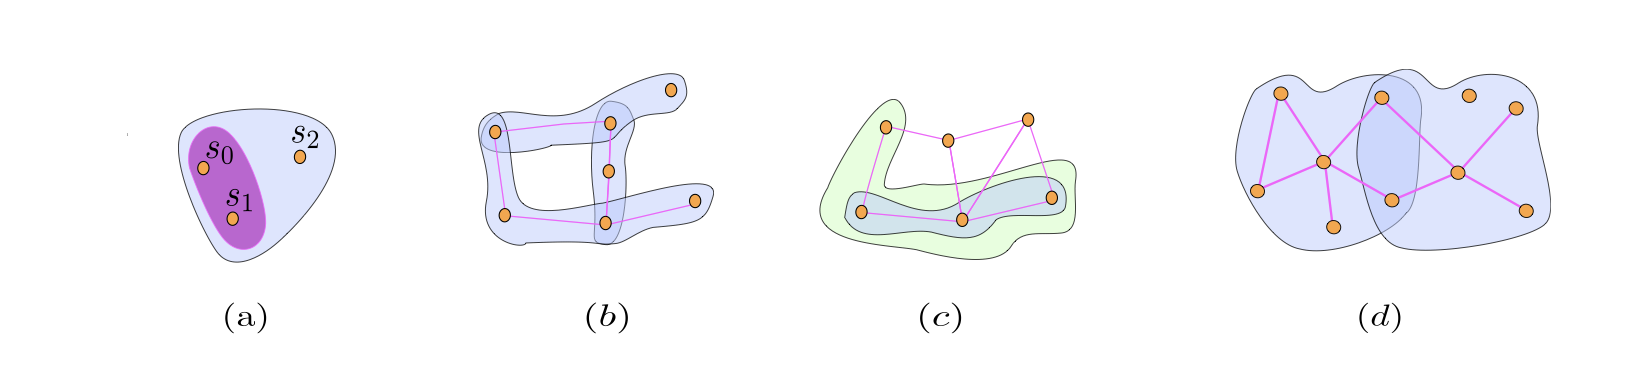
\includegraphics[width=0.9\textwidth]{images/combinatorial_complex.png}
\caption{\textbf{Combinatorial complexes generalise graphs by allowing cells of
several ranks.} Orange discs are vertices (rank-0 cells); pink, blue and green
regions are cells of rank 1, 2 and 3, each a set of vertices treated as a single
object. Examples (a), (b), (d) have dimension~2 and (c) has dimension~3. Adapted
from Hajij et al.~\cite{hoan}.}
\label{fig:cc-examples}
\end{figure}

\subsection{Neighborhood functions}

A CC carries \emph{neighborhood functions} $\mathcal{N}$ (Def.~12 of~\cite{hoan}),
which assign to a cell the set of cells in its local vicinity. Two are used here.
Two cells are \emph{incident} when one strictly contains the other; the down- and
up-incidence functions of a cell $x$ are
\[
\mathcal{N}_{\downarrow}(x)=\{y\in\mathcal{X}\mid y\subsetneq x\},\qquad
\mathcal{N}_{\uparrow}(x)=\{y\in\mathcal{X}\mid x\subsetneq y\},
\]
linking cells of different ranks (a residue and the helix that contains it). Two
same-rank cells are \emph{adjacent} when they share a bridge cell of higher rank
(Def.~17). A neighborhood function is stored as a binary neighborhood matrix; in
particular the \emph{incidence matrix}
$B_{r,k}\in\{0,1\}^{|\mathcal{X}^{r}|\times|\mathcal{X}^{k}|}$ has $[B_{r,k}]_{ij}=1$
when the $r$-cell $x^{r}_i$ is incident to the $k$-cell $x^{k}_j$. Each $B_{r,k}$
induces a cochain map $B_{r,k}:C^{k}(\mathcal{X})\to C^{r}(\mathcal{X})$ (Def.~22),
the discrete operator that moves signals between ranks.

\begin{figure}[h]
\centering
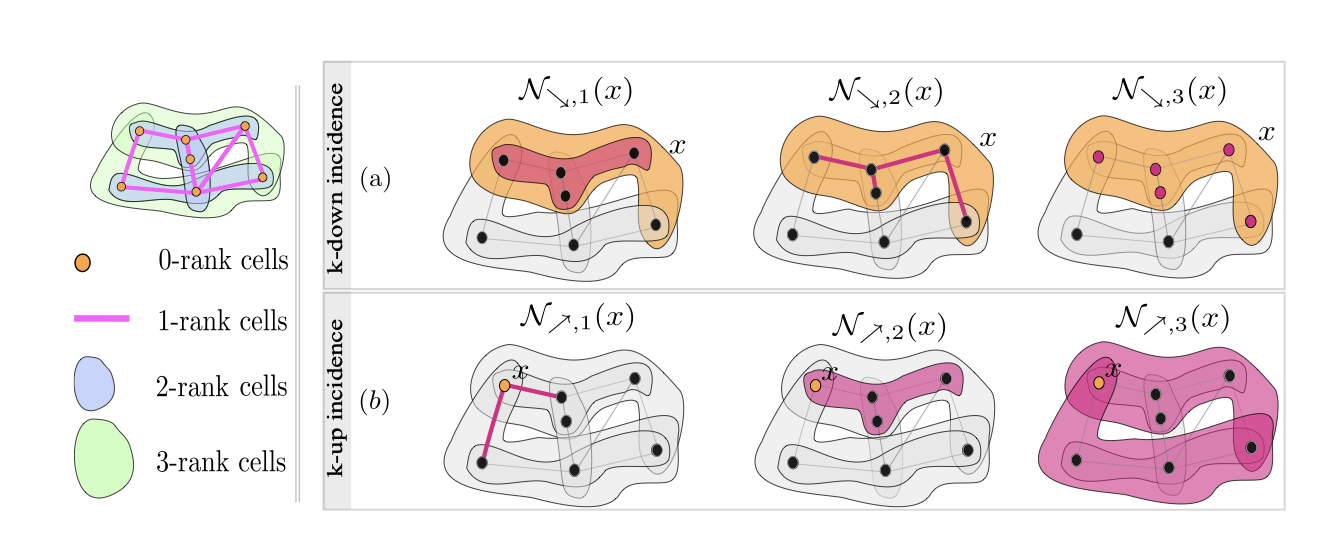
\includegraphics[width=0.92\textwidth]{images/neighborhood_functions.png}
\caption{\textbf{Incidence neighborhood functions on a complex of dimension three}
(cells coloured by rank, key at left). Top: the $k$-down incidences
$\mathcal{N}_{\downarrow,1},\mathcal{N}_{\downarrow,2},\mathcal{N}_{\downarrow,3}$ of a
target cell $x$ --- the cells one, two and three ranks below that $x$ contains.
Bottom: the $k$-up incidences $\mathcal{N}_{\uparrow,k}$ of a vertex $x$ --- the
higher-rank cells that contain it. Adapted from Hajij et al.~\cite{hoan}.}
\label{fig:neigh}
\end{figure}

\subsection{Cochains and higher-order message passing}

Data live on cells as \emph{cochains}. The $k$-cochain space
$C^{k}(\mathcal{X},\mathbb{R}^{d})$ is the space of maps $H_k:\mathcal{X}^{k}\to
\mathbb{R}^{d}$ (Def.~21 of~\cite{hoan}); ordering the $k$-cells identifies it with
$\mathbb{R}^{|\mathcal{X}^{k}|\times d}$, and we write $H_k=[h_{x^{k}_1},\dots]$ with
$H_{k,j}=h_{x^{k}_j}$ the feature of cell $x^{k}_j$. A CCNN layer updates the
cochains by \emph{higher-order message passing} over a set
$\mathcal{N}=\{\mathcal{N}_1,\dots,\mathcal{N}_n\}$ of neighborhood functions
(Def.~34): for a cell $x$ and a layer index $l$,
\[
 m_{x,y}=\alpha_{\mathcal{N}_k}\!\big(h_x^{(l)},h_y^{(l)}\big),\qquad
 m_x^{k}=\bigoplus_{y\in\mathcal{N}_k(x)} m_{x,y},\qquad
 m_x=\bigotimes_{\mathcal{N}_k\in\mathcal{N}} m_x^{k},\qquad
 h_x^{(l+1)}=\beta\!\big(h_x^{(l)},m_x\big),
\]
where $\bigoplus$ is a permutation-invariant \emph{intra-neighborhood} aggregation,
$\bigotimes$ the \emph{inter-neighborhood} aggregation over the chosen
neighborhoods, and $\alpha_{\mathcal{N}_k},\beta$ are differentiable. When the
messages are attention-weighted --- a combinatorial complex attention network
(CCANN, Def.~31--33) --- the weight of neighbour $y$ is
$\mathrm{att}(x,y)=e_{xy}\big/\!\sum_{y'\in\mathcal{N}_k(x)}e_{xy'}$, a distribution
over $\mathcal{N}_k(x)$. This is the mechanism the model uses, with the
neighborhoods given by the incidence functions of the PCC.

\begin{figure}[h]
\centering
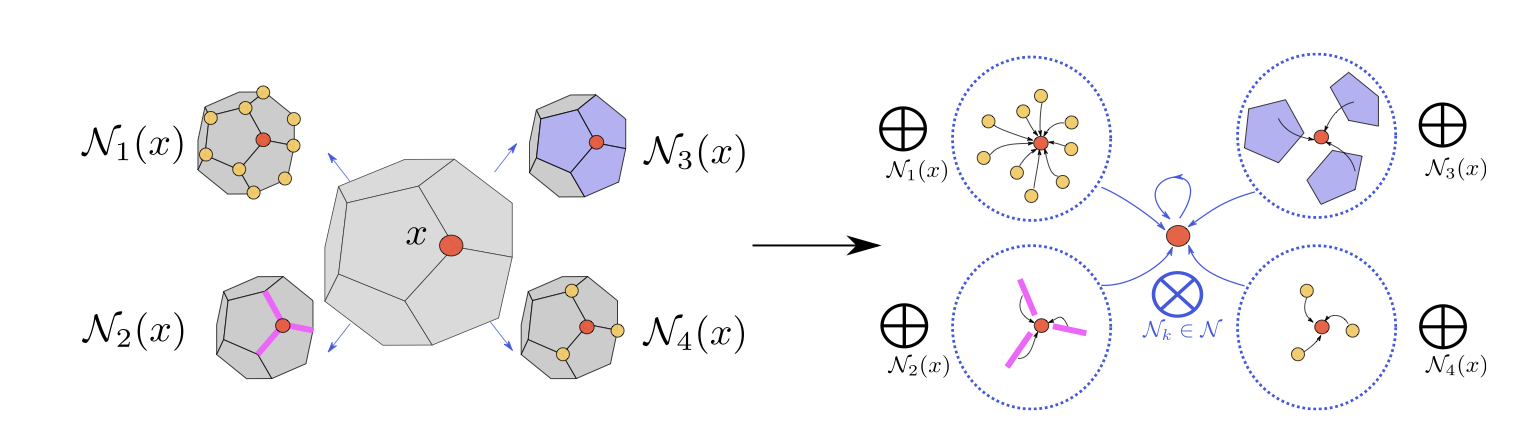
\includegraphics[width=0.95\textwidth]{images/message_passing.png}
\caption{\textbf{One step of higher-order message passing (Def.~34).} Left: for the
target cell $x$, several neighborhood functions $\mathcal{N}_1,\dots,\mathcal{N}_k$
are selected (different incidence or adjacency relations). Right: inside each
neighborhood the incoming messages are combined by the intra-neighborhood
aggregation $\bigoplus$; the results from all neighborhoods are then merged by the
inter-neighborhood aggregation $\bigotimes$ and used to update $x$. Adapted from
Hajij et al.~\cite{hoan}.}
\label{fig:homp}
\end{figure}

\subsection{Permutation equivariance}

Let $P_k$ be a permutation matrix that relabels the $k$-cells. If every cochain is
relabelled, $H_k\mapsto P_kH_k$, and every incidence matrix accordingly,
$B_{r,k}\mapsto P_rB_{r,k}P_k^{\top}$, then a CCNN layer commutes with the
relabelling, and its output transforms as $H_k'\mapsto P_kH_k'$. CCNNs are
therefore permutation-equivariant, the higher-order analogue of the permutation
equivariance of GNNs. A protein-level prediction is made permutation-invariant by
ending with a symmetric pooling over cells.

\section{The Protein Combinatorial Complex}
\label{sec:pccnn}

Topotein~\cite{topotein} instantiates the framework of
Section~\ref{sec:ccnn} for proteins. The Protein Combinatorial Complex (PCC) of a
protein is a CC $(S,\mathcal{X},\mathrm{rk})$ of dimension $\dim(\mathcal{X})=3$
whose entities $S$ are the residues, with cells of four ranks: the residues
themselves ($\mathcal{X}^{0}$), the spatial contacts ($\mathcal{X}^{1}$), the
secondary-structure elements (SSEs, $\mathcal{X}^{2}$), and a single cell for the
whole protein ($\mathcal{X}^{3}$). The incidence functions used are those recorded
by $B_{0,1}$ (which residues form each contact), $B_{0,2}$ (which residues compose
each SSE), and $B_{0,3},B_{2,3}$ (that every residue and SSE lies in the protein
cell).

Each rank carries two cochains, a scalar cochain and a vector cochain, transforming
under two representations of $SO(3)$: the scalar $\mathbf{s}_{x}\in\mathbb{R}^{n_r}$
under the trivial representation (it is \emph{invariant}), the vector
$\mathbf{V}_{x}\in\mathbb{R}^{m_r\times 3}$ under the standard representation (it is
\emph{equivariant}, $\mathbf{V}_{x}\to\mathbf{V}_{x}R^{\top}$ for $R\in SO(3)$). The
encoder (Section~\ref{sec:architecture}) preserves both transformation laws at every
layer; the final readout is a scalar, hence SE(3)-invariant, and
permutation-invariant after pooling --- the property clustering requires.

\subsection{Neighborhood functions of the PCC}
\label{sec:pcc-neigh}

Message passing on the PCC uses the incidence and adjacency neighborhoods of
Section~\ref{sec:ccnn}, in the directed form of Topotein~\cite{topotein}. Following
their notation, $B^{r\to r'}\in\{0,1\}^{|\mathcal{X}^{r'}|\times|\mathcal{X}^{r}|}$
is the incidence matrix routing a rank-$r$ cochain to rank $r'$; it is the
$B_{r,r'}$ (or its transpose) of Section~\ref{sec:ccnn} read as a directed map.

\paragraph{Directed $1$-cells.} Unlike the undirected hyperedges of the general
combinatorial complex, the PCC's $1$-cells are \emph{directed} pairwise edges. For
an edge $(i,j)$, only the source $i$ pushes to the edge (via $B^{0\to1}$) and the
edge pushes only to the target $j$ (via $B^{1\to0}$). This orientation is what makes
the SO(3)-equivariant edge frames of Section~\ref{sec:architecture} well defined.

\paragraph{Outer-edge neighborhoods.} Each residue belongs to exactly one SSE, so
the $2$-cells never overlap and cannot communicate through ordinary down-adjacency
(they would only echo messages back to themselves). To let SSEs exchange
information, Topotein defines \emph{outer-edge neighborhoods}
\[
N^{2\to1}_{\mathrm{outer}}=B^{2\to0}\!\cdot B^{0\to1}-B^{2\to1},\qquad
\big(N^{1\to2}_{\mathrm{outer}}\big)^{\top}=B^{2\to0}\!\cdot\big(B^{1\to0}\big)^{\top}-B^{2\to1},
\]
where $B^{2\to1}$ is the set of \emph{inner} edges (both endpoints inside one SSE).
Thus $N^{2\to1}_{\mathrm{outer}}$ maps an SSE to the edges that \emph{start} inside
it but \emph{end} in a different SSE, and $(N^{1\to2}_{\mathrm{outer}})^{\top}$ to
those that end inside it but start elsewhere: exactly the inter-SSE contacts, with
one edge per contact so no geometric information is lost. These are the channels
that carry tertiary packing (which strands pair, which helices pack) between
secondary structures.

\begin{figure}[h]
\centering
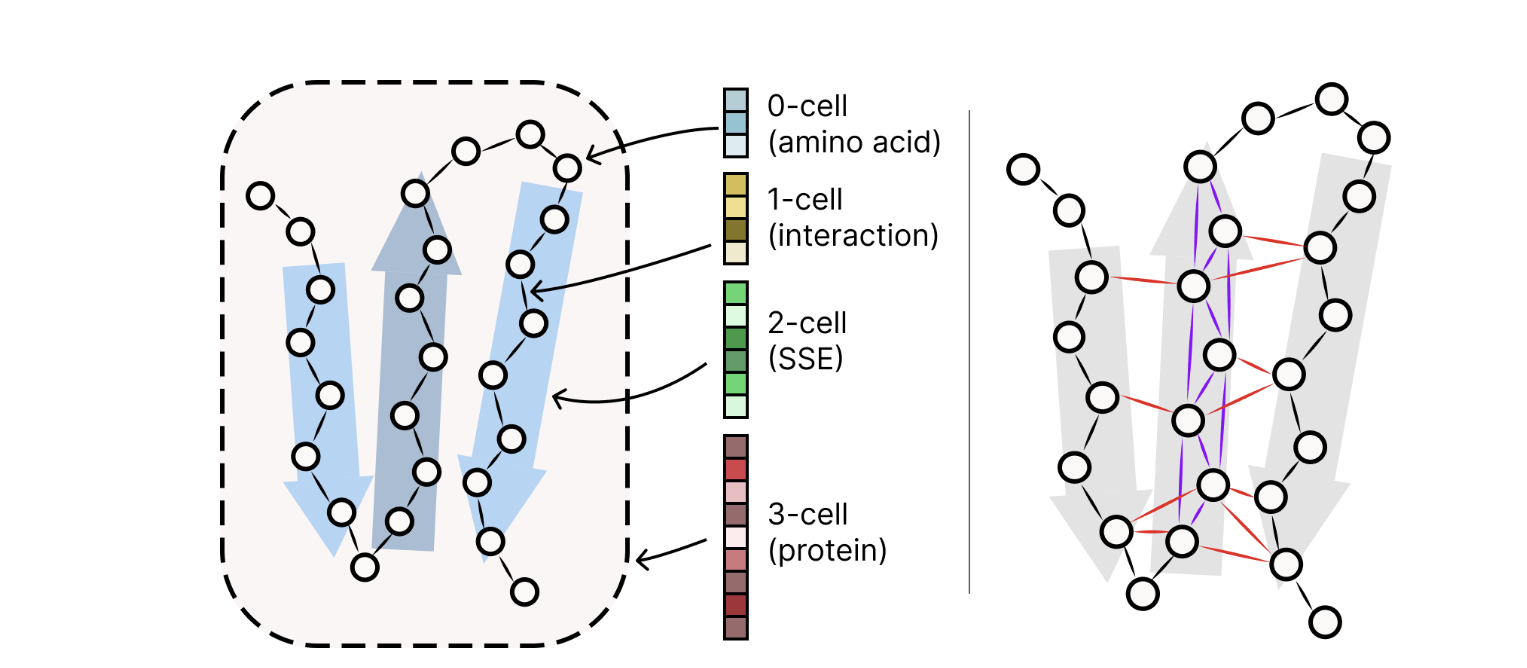
\includegraphics[width=0.92\textwidth]{images/PCC.png}
\caption{\textbf{The Protein Combinatorial Complex (PCC).} Left: a protein as a
four-rank complex --- amino-acid nodes (0-cells, black circles), interaction edges
(1-cells, black lines), secondary-structure elements (2-cells, blue arrows) and the
whole protein (3-cell, dashed box); the colour key gives the rank of each cell.
Right: inner edges (purple) lie inside a single SSE, whereas outer edges (red)
connect two \emph{different} SSEs --- these are the contacts the outer-edge
neighborhoods $N^{2\to1}$ use to pass messages between secondary structures. Adapted
from Topotein~\cite{topotein}.}
\label{fig:pcc}
\end{figure}

\subsection{Featurization}
\label{sec:featurization}
\label{sec:lifting}

Featurization (``lifting'') turns a predicted structure into a PCC, once per
protein and offline. Only the C$\alpha$ trace $\mathbf{c}_1,\dots,\mathbf{c}_N\in
\mathbb{R}^{3}$ of the first chain is used; every feature below is a function of
these coordinates, so all scalar features are rigid-motion invariant and the sole
raw vector feature is a displacement. Write $N$ for the number of residues, $k=16$
the graph degree, $E=kN$ the number of directed edges, and $S$ the number of SSEs.
For an edge $e$, $\mathrm{s}(e)$ and $\mathrm{t}(e)$ are its source and target
residues; $\sigma(i)\in\{1,\dots,S\}$ is the SSE of residue $i$; when proteins are
batched, $\beta(i)$ and $\beta_2(p)$ map a residue or SSE to its protein. These
maps are the incidence relations $B_{0,1},B_{0,2},B_{0,3},B_{2,3}$ read as
functions.

\paragraph{Rank 0 --- residues.} The scalar feature is the backbone dihedral pair,
sine/cosine encoded so the angle wraps smoothly:
\[
\mathbf{s}^{0}_i=(\sin\phi_i,\cos\phi_i,\sin\psi_i,\cos\psi_i)\in\mathbb{R}^{4}.
\]
Residues carry no amino-acid identity, no 3Di token and no sequence-position
encoding; the only other per-residue datum is the coordinate $\mathbf{c}_i$, which
seeds the vector channels and the local frames of Section~\ref{sec:architecture}.

\paragraph{Rank 1 --- contacts.} A directed $k$-nearest-neighbour graph on the
C$\alpha$ atoms ($k=16$, the self-neighbour excluded). Edge $e$ from $i=\mathrm{s}(e)$
to $j=\mathrm{t}(e)$ carries a scalar and a vector,
\[
d_e=\lVert\mathbf{c}_j-\mathbf{c}_i\rVert,\qquad
\mathbf{s}^{1}_e=[\,d_e\,\|\,\mathrm{RBF}(d_e)\,]\in\mathbb{R}^{1+K},\qquad
\mathbf{v}^{1}_e=\mathbf{c}_j-\mathbf{c}_i\in\mathbb{R}^{1\times 3},
\]
where $\mathbf{v}^{1}_e$ is the only raw vector feature in the complex and
$\mathrm{RBF}(\cdot)$ is a radial-basis expansion of the distance (specified in a
later iteration).

\paragraph{Ranks 2 and 3 --- SSEs and protein.} Residues receive a PSEA
three-state label (helix, strand, loop); maximal runs of one label form the SSEs,
and $\sigma(i)$ records membership. A point set $\{\mathbf{c}_i\}_{i=1}^{m}$ (the
residues of one SSE for rank 2, the whole chain for rank 3) with centroid
$\bar{\mathbf{c}}$ is summarised by the covariance and its spectrum,
\[
\Sigma=\frac{1}{m-1}\sum_{i=1}^{m}(\mathbf{c}_i-\bar{\mathbf{c}})(\mathbf{c}_i-\bar{\mathbf{c}})^{\top}
=\sum_{a=1}^{3}\lambda_a\,\mathbf{u}_a\mathbf{u}_a^{\top},\quad
\lambda_1\ge\lambda_2\ge\lambda_3\ge 0,
\]
giving five scale-normalised shape descriptors
\[
\Big(\tfrac{\lambda_1-\lambda_2}{\lambda_1},\
\tfrac{2(\lambda_2-\lambda_3)}{\lambda_1+\lambda_2},\
\tfrac{3\lambda_3}{\lambda_1+\lambda_2+\lambda_3},\
\operatorname{sign}(\textstyle\prod_a\lambda_a)\,|\textstyle\prod_a\lambda_a|^{1/3},\
\tfrac{\lambda_1-\lambda_3}{\lambda_1}\Big).
\]
The rank-2 scalar feature is the SSE type one-hot ($4$, with a catch-all slot),
these five descriptors, and the three eigenvalues,
$\mathbf{s}^{2}_p\in\mathbb{R}^{12}$. The single rank-3 scalar feature stacks the
size $N$, the radius of gyration $R_g=\big(\tfrac1N\sum_i\lVert\mathbf{c}_i-\bar{\mathbf{c}}\rVert^2\big)^{1/2}$,
and the five descriptors and three eigenvalues of the whole chain,
$\mathbf{s}^{3}\in\mathbb{R}^{10}$. All of these are functions of interatomic
distances only, hence invariant to rotation and translation. Ranks 1--3 have no
raw vector feature; their vector channels are seeded from $\mathbf{v}^{1}$ in
Section~\ref{sec:embed}.

\subsection{Train / validation split}
\label{sec:split}

The split is cluster-aware and leakage-controlled, built once from the featurized
pool. First, a small set of downstream control proteins is held out into a separate
manifest and excluded from both train and validation. Second, the structures are
grouped into their Foldseek structural clusters, and whole clusters are assigned
entirely to train \emph{or} to validation (a \emph{cold} split), so no structural
cluster --- and hence no group of near-duplicate folds --- spans the two sets.
Finally, each cluster is subsampled at a common rate
$f=\text{target}/\text{pool}\approx 0.214$, which scales every cluster (singletons
included) by the same factor and so preserves the cluster-size distribution at the
target size. The resulting split is disjoint at the level of structural clusters,
and here yields $3{,}191$ train and $813$ validation proteins. Family labels are
used only to evaluate the embeddings, never during training.

\begin{figure}[h]
\centering
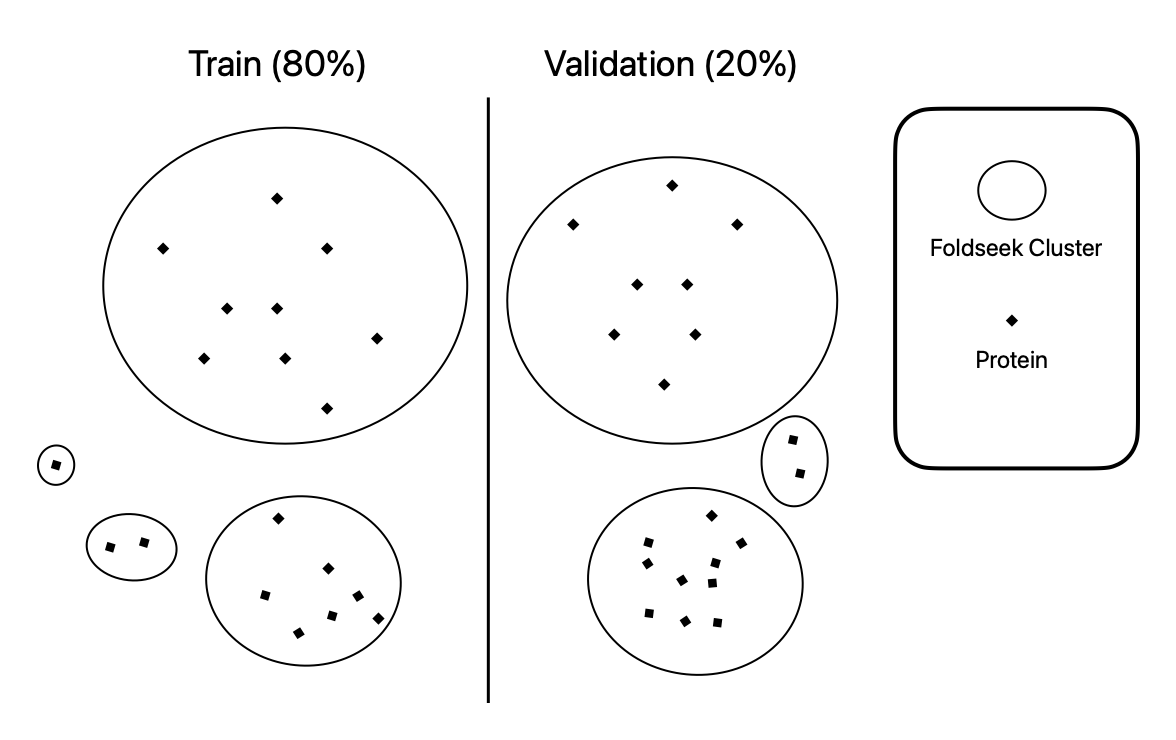
\includegraphics[width=0.82\textwidth]{images/cold_cluster_split.png}
\caption{\textbf{Leakage-controlled cold cluster split.} Each ellipse is a Foldseek
structural cluster and each diamond a protein. Whole clusters --- not individual
proteins --- are assigned to train ($\sim$80\%) or validation ($\sim$20\%), so no
structural cluster spans the split and no near-duplicate fold can leak from one set
to the other. Each cluster is then subsampled at the common rate $f$}
\end{figure}

\section{Architecture}
\label{sec:architecture}

The encoder is the Topology-Complete Perceptron Network (TCPNet) of
Topotein~\cite{topotein}: an SE(3)-equivariant CCANN
(Section~\ref{sec:ccnn}) on the PCC. It processes scalar and vector cochains at
every rank through the Topology-Complete Perceptron (TCP) module, with an embedding
stage, $L$ interaction layers of four-step hierarchical message passing, and a
readout. We describe the full architecture faithfully; the one degree of freedom we
add is that the \emph{order} of the message-passing steps is made configurable
through a tensor-diagram flag (Section~\ref{sec:modular}). A batch holds $B$
proteins; after embedding, the feature of a cell $x^{r}$ is a pair
$(\mathbf{s}_x,\mathbf{V}_x)$ of scalar width $d_s$ and vector width $d_v$, collected
into the cochain $H_r$.

\subsection{Edge-centric frames and scalarization}
\label{sec:frames}

Vector features enter the invariant scalar stream only through projection onto local
orthonormal frames. Topotein uses \emph{edge-centric} frames: for the directed edge
$(i,j)$ with C$\alpha$ positions $\mathbf{x}_i,\mathbf{x}_j$,
\[
\mathbf{F}_{(i,j)}=\Big(\tfrac{\mathbf{x}_j-\mathbf{x}_i}{\lVert\mathbf{x}_j-\mathbf{x}_i\rVert},\;
\tfrac{\mathbf{x}_j\times\mathbf{x}_i}{\lVert\mathbf{x}_j\times\mathbf{x}_i\rVert},\;
\tfrac{\mathbf{x}_j-\mathbf{x}_i}{\lVert\mathbf{x}_j-\mathbf{x}_i\rVert}\times\tfrac{\mathbf{x}_j\times\mathbf{x}_i}{\lVert\mathbf{x}_j\times\mathbf{x}_i\rVert}\Big)\in\mathbb{R}^{3\times 3},
\]
translation-invariant and rotation-equivariant ($\mathbf{F}_{(i,j)}\to\mathbf{F}_{(i,j)}R^{\top}$),
with the cross-product axis flipping under reflection so the projection is
chirality-sensitive. The scalarization $S^{(r)}_i(\cdot)$ of a cell's vector feature
is the flattened projection onto the relevant frame(s), aggregated per rank:
\[
\begin{aligned}
\text{edge }(i,j):\quad & S_{(i,j)}\big(\mathbf{h}^{(1)}_{(i,j),v}\big)=\mathrm{flatten}\big(\mathbf{h}^{(1)}_{(i,j),v}\cdot\mathbf{F}_{(i,j)}\big),\\[2pt]
\text{residue }i:\quad & S_i\big(\mathbf{h}^{(0)}_{i,v}\big)=\mathrm{flatten}\Big(\tfrac{1}{|B^{0\to1}_i|}\!\!\sum_{(i,j)\in B^{0\to1}_i}\!\!\mathbf{h}^{(0)}_{i,v}\cdot\mathbf{F}_{(i,j)}\Big),\\[2pt]
\text{SSE }i:\quad & S_i\big(\mathbf{h}^{(2)}_{i,v}\big)=\mathrm{flatten}\Big(\tfrac{1}{|N^{2\to1}_i|}\!\!\sum_{(l,j)\in N^{2\to1}_i}\!\!\mathbf{h}^{(2)}_{i,v}\cdot\mathbf{F}_{(l,j)}\Big),
\end{aligned}
\]
i.e.\ residue vectors are read in the frames of their incident edges ($B^{0\to1}$)
and SSE vectors in the frames of their outer edges ($N^{2\to1}$,
Section~\ref{sec:pcc-neigh}). The protein ($r=3$) frame is not edge-based --- there
are no inter-protein edges --- but the three principal eigenvectors
$\mathbf{F}^{(3)}=(\mathbf{v}_1,\mathbf{v}_2,\mathbf{v}_3)$ of the C$\alpha$ point
cloud, sign-disambiguated by the farthest-residue anchor of Bro et al.~\cite{bro2008}.

\subsection{The Topology-Complete Perceptron (TCP)}
\label{sec:tcp}

The TCP module~\cite{topotein} is the rank-agnostic generalisation of the
Geometry-Complete Perceptron~\cite{gcpnet}: it maps a $(\mathbf{h}_s,\mathbf{h}_v)$
pair, $\mathbf{h}_s\in\mathbb{R}^{d_s}$, $\mathbf{h}_v\in\mathbb{R}^{d_v\times 3}$,
to updated scalar and vector features using the rank-$r$ frame. Two bias-free MLPs
$V_s,V_d$ reduce the vector channels, the reduced vectors are scalarized and
concatenated with the scalars, and dedicated MLPs $S_{\mathrm{out}},V_u$ with a
scalar gate produce the outputs:
\[
\begin{aligned}
\mathbf{s}=\sigma\big(V_s(\mathbf{h}_v)\big)\in\mathbb{R}^{3\times 3},\qquad
&\mathbf{z}=\sigma\big(V_d(\mathbf{h}_v)\big)\in\mathbb{R}^{(d_v/\lambda)\times 3},\\
\mathbf{h}'_s=\big(\mathbf{h}_s,\;S^{(r)}_i(\mathbf{s}),\;\lVert\mathbf{z}\rVert_2\big)\in\mathbb{R}^{d_s+9+d_v/\lambda},\qquad
&\mathbf{h}_{s,\mathrm{out}}=\sigma\big(S_{\mathrm{out}}(\mathbf{h}'_s)\big)\in\mathbb{R}^{d_s},\\
\mathbf{h}'_v=\sigma\big(V_u(\mathbf{z})\big)\in\mathbb{R}^{d_v\times 3},\qquad
&\mathbf{h}_{v,\mathrm{out}}=\mathbf{h}'_v\odot\sigma_g\big(S_{\mathrm{gate}}(\mathbf{h}_{s,\mathrm{out}})\big),
\end{aligned}
\]
where $\lambda$ is the bottleneck factor, $\odot$ the element-wise product and
$\sigma_g$ a sigmoid gate that keeps the vector output equivariant while letting the
scalars modulate its magnitude. The scalarization $S^{(r)}_i$ is what lets a single
module process residues, edges, SSEs and the protein cell uniformly while preserving
SE(3)-equivariance. We write $\mathrm{TCP}^{(r)}$ for the module at rank $r$.

\subsection{Embedding module}
\label{sec:embed}

Raw features are first stabilised by GVP layer normalisation~\cite{gvp} (which
normalises scalars and rescales vectors by their mean norm) and then mapped to the
common width $(d_s,d_v)$ by rank-specific TCP modules:
\[
H^{(r)}=\varphi^{(r)}_{\mathrm{emb}}\big(\mathrm{LN}(H^{(r)}_0)\big),\qquad r\in\{0,1,2,3\},
\]
where $H^{(r)}_0$ are the raw cochains of Section~\ref{sec:featurization}. Since the
featurization stores a raw \emph{vector} feature only on the edges
($\mathbf{v}^{1}_e$, the displacement), the residue, SSE and protein vector channels
are seeded from it by mean aggregation up the ranks ($\mathbf{v}^{0}_i=\tfrac1k\sum_{e:\mathrm{s}(e)=i}\mathbf{v}^{1}_e$,
then averaged into SSEs and the protein) before the embedding TCP.

\subsection{Hierarchical message passing}
\label{sec:attention}

Each interaction layer runs Topotein's four-step scheme, a bottom-up-then-down
sweep in which edges, SSEs, residues and the protein cell are updated in turn;
$\bigoplus$ denotes a permutation-invariant aggregation and every message/update
function $\phi^{(r)}$ is a TCP module (Section~\ref{sec:tcp}).

\paragraph{Step 1 --- edge messages.} Each edge integrates its source and target
residues, its own feature, and the SSE features of both endpoints, then applies a
TCP residual and a scalar-attention gate:
\[
\mathbf{m}_{ij}=\phi^{(1)}\big(\mathbf{h}^{(0)}_i,\mathbf{h}^{(0)}_j,\mathbf{h}^{(1)}_{ij},\mathbf{n}_i,\mathbf{n}_j\big),\qquad
\mathbf{n}_i=\begin{cases}\mathbf{h}^{(2)}_k & \exists\,k\in\mathcal{X}^{2},\ i\in k\\ \mathbf{0} & \text{otherwise,}\end{cases}
\]
\[
\mathbf{h}^{l+1}_{ij}=\phi_{\mathrm{msg}}\big(\mathbf{h}^{l}_{ij}\big)+\mathbf{h}^{l}_{ij},\qquad
\mathbf{m}_{ij}=\big(\mathbf{h}^{\mathrm{fin}}_{ij,s}\odot\sigma_{\mathrm{att}}(\mathbf{w}^{\top}\mathbf{h}^{\mathrm{fin}}_{ij,s}),\ \mathbf{h}^{\mathrm{fin}}_{ij,v}\big).
\]

\paragraph{Step 2 --- SSE update.} Each SSE aggregates its constituent residues
($B^{2\to0}$), its inner edges ($B^{2\to1}$) and, crucially, the edge messages of
its outer-edge neighborhood ($N^{2\to1}$, the inter-SSE channel):
\[
\mathbf{u}^{(2)}_i=\phi^{(2)}\Big(\mathbf{h}^{(2)}_i,\ \bigoplus_{j\in B^{2\to0}_i}\mathbf{h}^{(0)}_j,\ \bigoplus_{j\in B^{2\to1}_i}\mathbf{h}^{(1)}_j,\ \bigoplus_{(j,k)\in N^{2\to1}_i}\mathbf{m}_{jk}\Big).
\]

\paragraph{Step 3 --- residue refinement.} Each residue is refined from its parent
SSE and its incoming edge messages:
\[
\mathbf{u}^{(0)}_i=\phi^{(0)}\Big(\mathbf{h}^{(0)}_i,\ \mathbf{m}^{(2)}_i,\ \bigoplus_{j\in(B^{1\to0}_i)^{\top}}\mathbf{m}_{ji}\Big),\qquad
\mathbf{m}^{(2)}_i=\begin{cases}\mathbf{u}^{(2)}_k & \exists\,k\in\mathcal{X}^{2},\ i\in k\\ \mathbf{0} & \text{otherwise.}\end{cases}
\]

\paragraph{Step 4 --- protein update.} The global cell aggregates the updated
residues and SSEs:
\[
\mathbf{u}^{(3)}_i=\phi^{(3)}\big(\mathbf{u}^{(0)}_i,\mathbf{u}^{(2)}_i,\mathbf{h}^{(3)}_i\big).
\]

\paragraph{Feature update.} Ranks $\{0,2,3\}$ are updated with a residual and layer
normalisation (rank 1 is already updated in Step 1):
\[
\mathbf{h}^{(r)\prime}_i=\mathrm{LN}\big(\mathbf{u}^{(r)}_i+\mathbf{h}^{(r)}_i\big),\qquad r\in\{0,2,3\}.
\]
The stack applies $L$ such layers. Because every attention weight is an invariant
scalar and every function is a TCP, scalars stay SE(3)-invariant and vectors
SO(3)-equivariant throughout. Note that, unlike the residue-hub simplifications,
this scheme couples rank 1 and rank 2 directly: SSE features enter edge messages
($\mathbf{n}_i,\mathbf{n}_j$ in Step 1) and edge messages update SSEs through the
outer-edge channel (Step 2).

\subsection{Modular ordering and the tensor-diagram flag}
\label{sec:modular}

Each of the four steps is a cochain push-forward (Section~\ref{sec:ccnn}) along a
chosen neighborhood set, and a layer is their ordered composition. A CCNN is
exactly specified by a \emph{tensor diagram} (Def.~24 of~\cite{hoan}): a directed
graph whose nodes are the cochains $C^{0}\!-\!C^{3}$ and whose labelled edges are the
push-forwards ($B^{0\to1}$, $B^{2\to0}$, $B^{2\to1}$, $N^{2\to1}$, $B^{1\to0}$,
$B^{0\to3}$, $B^{2\to3}$, and adjacencies such as $A^{2\sim1}$), meeting at merge
nodes where several messages reach the same target. Steps~1--4 above are one such
diagram, and it is the default.

We make this diagram a \emph{hyperparameter} of the training pipeline: the
interaction layer is built from a declarative tensor-diagram specification passed as
a flag (\texttt{-{}-tensor-diagram}), an ordered list of
$(\text{source ranks}\to\text{target rank},\ \text{neighborhood})$ steps. The
default reproduces TCPNet; alternative diagrams --- reordering the steps, inserting a
rank-2 adjacency $A^{2\sim1}$ so SSEs talk through shared contacts, dropping the
protein channel (replacing it by a pooling readout), or restricting to the residue
hub as a control --- are then swept without touching the model code
(Section~\ref{sec:plan}). The message-passing \emph{order} thus becomes an
experimental variable rather than a hard-coded choice.

\begin{figure}[h]
\centering
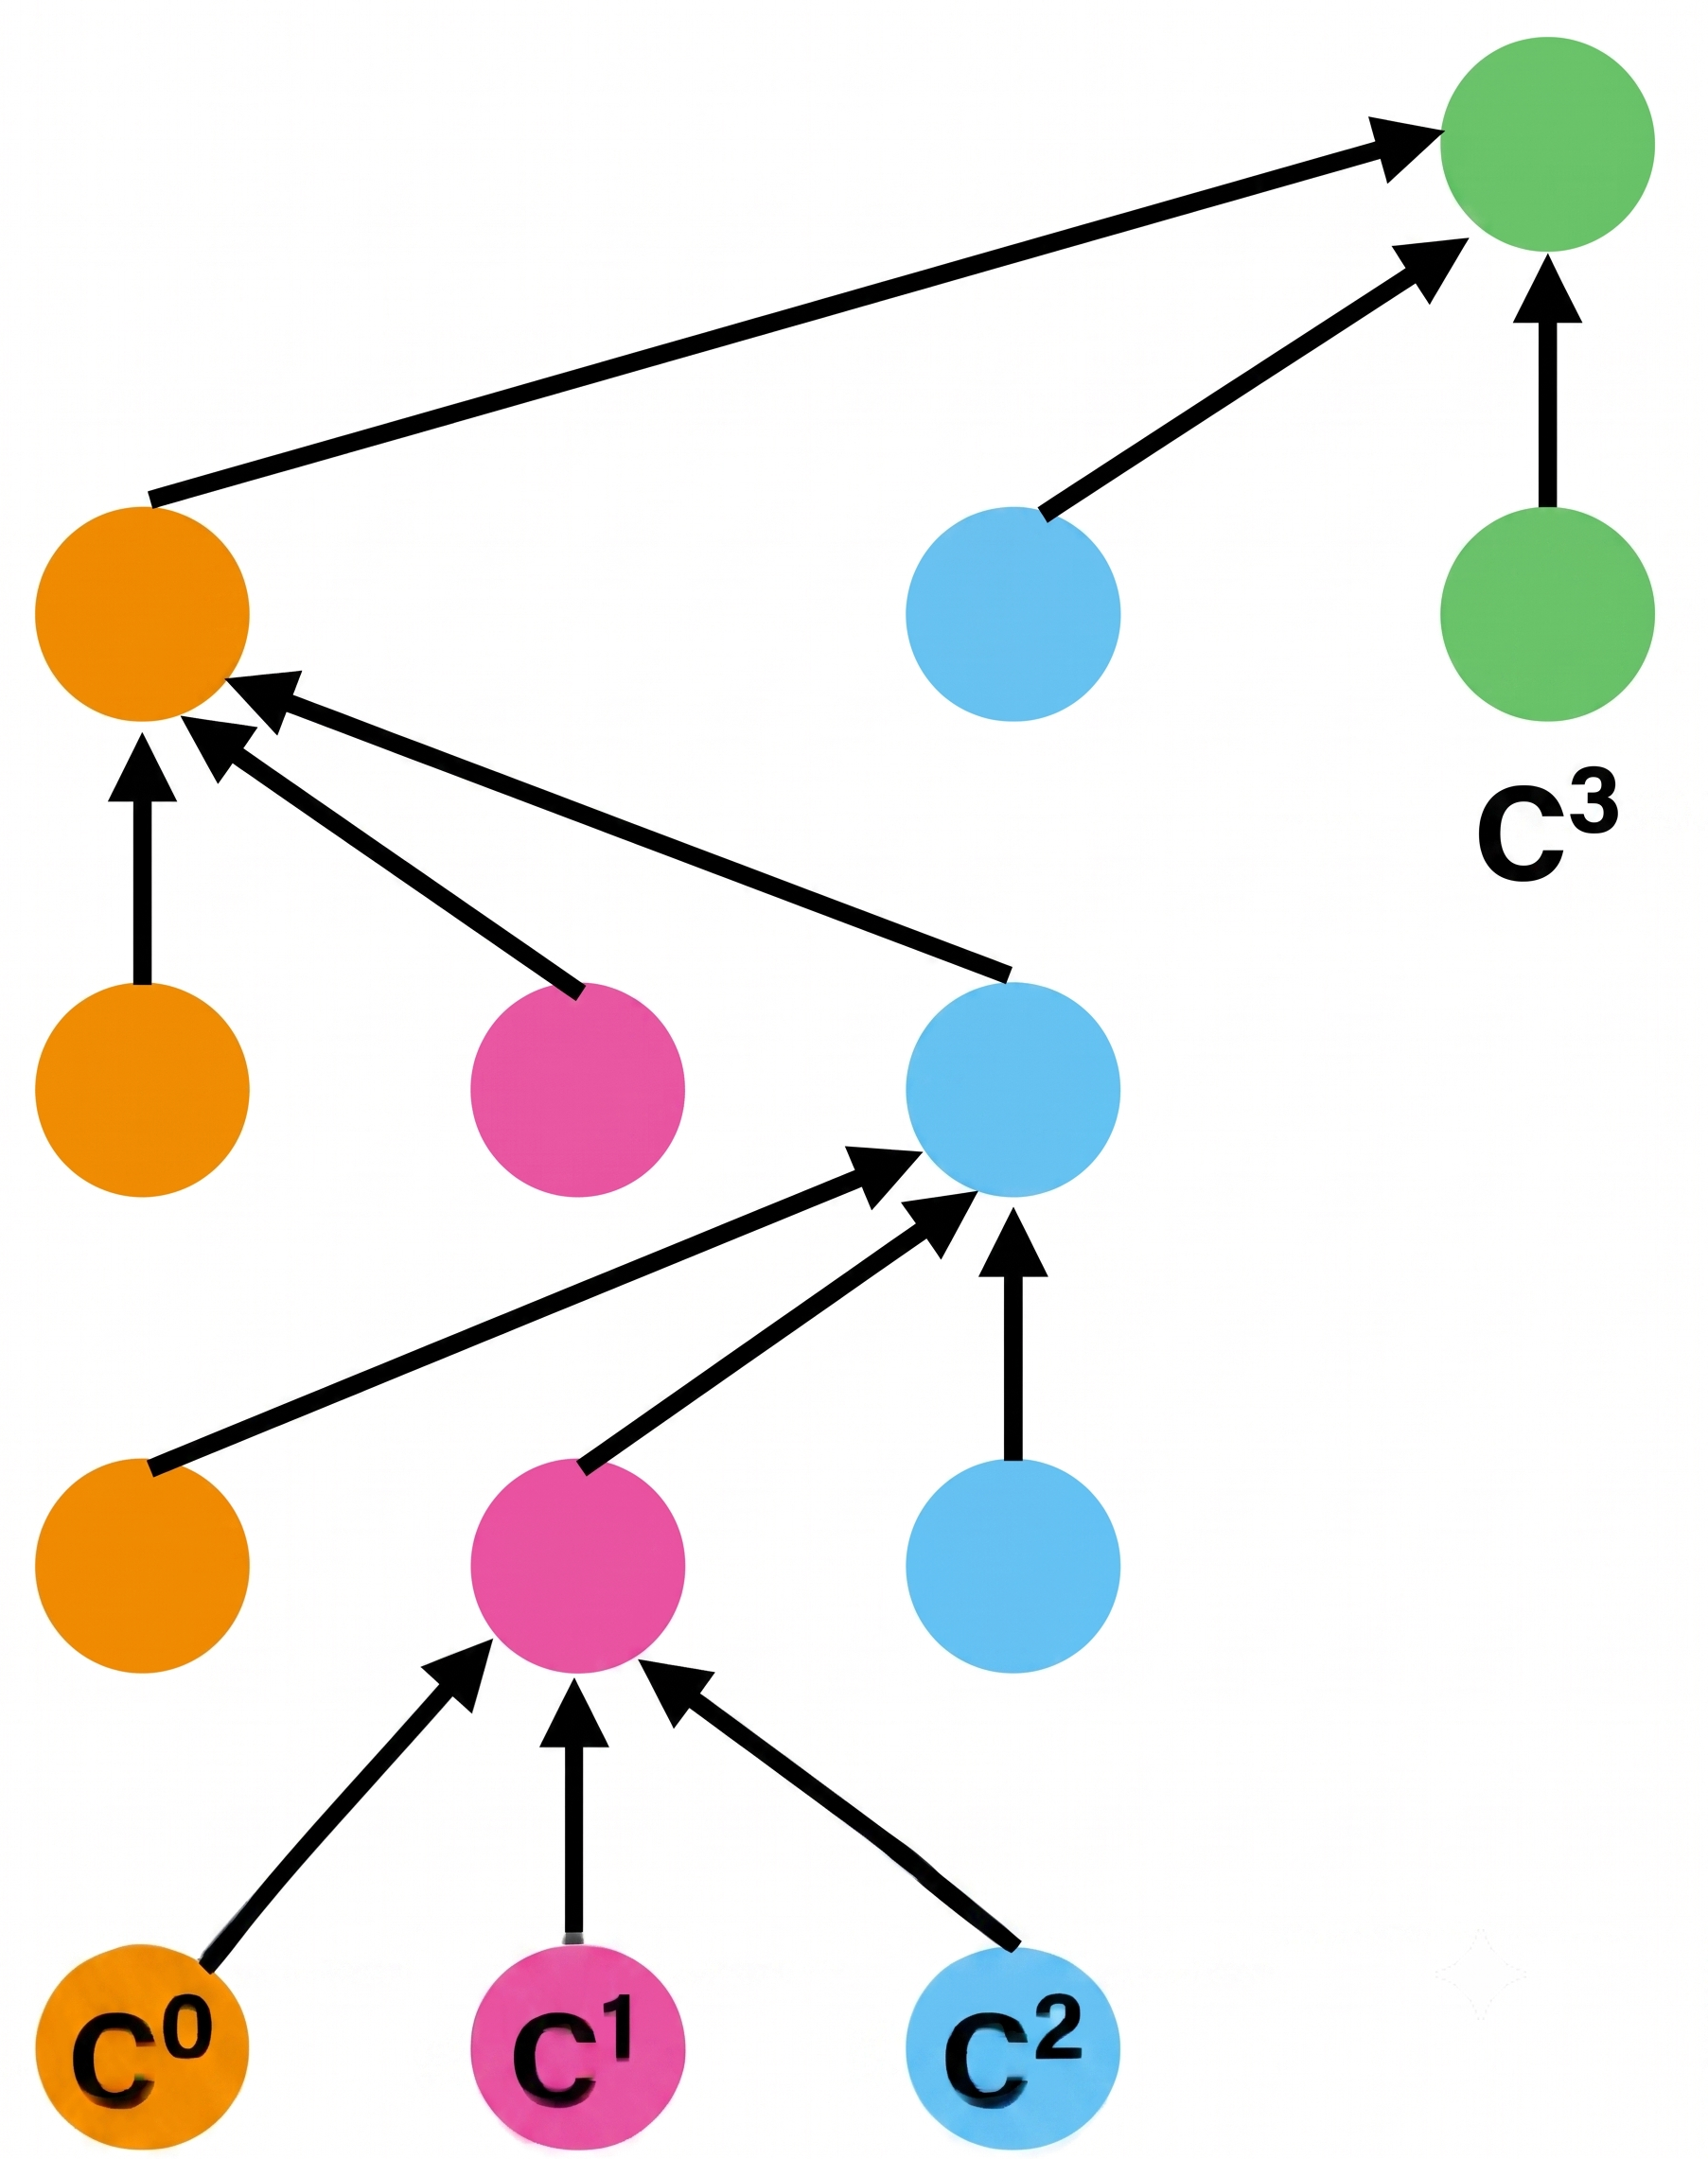
\includegraphics[height=8.2cm]{images/tensor_diagram.png}
\caption{\textbf{Tensor diagram of one interaction layer (Topotein default).} The
cochains $C^{0}$ (residues, orange), $C^{1}$ (edges, pink), $C^{2}$ (SSEs, blue) and
$C^{3}$ (protein, green) enter at the bottom; each arrow is a push-forward along an
incidence neighborhood and arrows meeting at a node are the merge that updates it.
Reading upward: edges gather from residues, edges and SSEs ($C^{0},C^{1},C^{2}\to
C^{1}$); SSEs update from residues, inner and outer edges ($\to C^{2}$); residues
refine from edges and their SSE ($\to C^{0}$); the protein pools residues and SSEs
($\to C^{3}$). This diagram is the object passed as the \texttt{-{}-tensor-diagram}
flag, so a different diagram gives a different message-passing order without changing
the model code.}
\end{figure}

\subsection{Readout and embedding}
\label{sec:readout}

Topotein offers two readouts, and we treat the choice as a flag. Either (i) the
final residue cochain $H^{(0)}$ is pooled (sum or mean) into a protein vector --- the
rank-3 message passing is then unused --- or (ii) the protein cochain $H^{(3)}$ is
used directly as the graph representation, which separates node- and graph-level
capacity but is more prone to over-fitting. In both cases the resulting scalar
representation $\mathbf{r}_b\in\mathbb{R}^{d_s}$ is $\ell_2$-normalised to
$\mathbf{z}_b=\mathbf{r}_b/\lVert\mathbf{r}_b\rVert\in\mathbb{S}^{d_s-1}$ and used
both for the contrastive loss (Section~\ref{sec:training}) and for evaluation. Since
the scalar stream is SE(3)-invariant and the pooling permutation-invariant,
$\mathbf{z}_b$ is invariant to rigid motion and residue reordering, and inverts under
reflection.


\subsection{Hyperparameters}

\begin{center}
\begin{tabular}{@{}l l l@{}}
\toprule
Group & Hyperparameter & Value\\
\midrule
Model & encoder                & TCPNet (TCP module, edge-centric frames)\\
      & scalar width $d_s$      & 128\\
      & vector width $d_v$      & 16\\
      & TCP bottleneck $\lambda$ & 3\\
      & interaction layers $L$  & 4\\
      & message-passing order   & Topotein 4-step (default; \texttt{-{}-tensor-diagram})\\
      & readout                 & node pooling (default) or protein cell\\
      & dropout                & 0.1\\
      & graph degree $k$       & 16\\
      & output dim             & 128, $\ell_2$-normalised\\
\midrule
Optim & optimizer              & AdamW\\
      & learning rate          & $1\times10^{-4}$\\
      & weight decay           & $1\times10^{-5}$\\
      & scheduler              & reduce-on-plateau (factor 0.5, patience 2)\\
      & gradient clip          & value clip 1.0\\
      & epochs                 & 50\\
      & batch size             & 256 proteins\\
\midrule
Loss  & objective              & InfoNCE / NT-Xent (in-batch negatives)\\
      & temperature $\tau$      & 0.2\\
      & positives               & two substructures, fraction $f\in[0.5,0.8]$\\
\bottomrule
\end{tabular}
\end{center}

\section{Training method}
\label{sec:training}

\subsection{What contrastive learning is}

The model is trained without any family labels, using contrastive learning. The
principle is simple: I take each protein and produce two \emph{views} of it, then I
train the encoder so that the two views of the same protein land close together in
the embedding space while views of different proteins are pushed apart. Over many
proteins, the only way to satisfy this everywhere is to place proteins that are
genuinely alike near each other and proteins that differ far apart. The encoder
therefore discovers, on its own, the features that make two proteins similar,
without ever being told what the families are. Two elements determine whether this
works: how the two views are made (the positive pair) and where the negatives come
from. The rest of this section specifies both.

There are two useful ways to read this objective. First, in information terms, the
two views are two partial observations of the same underlying structure, and the
contrastive loss is a lower bound on the mutual information between their
embeddings~\cite{infonce}: maximising it forces the embedding to keep exactly what
is common to both views (the fold) and to discard what differs between them (the
particular region sampled). Second, on the unit sphere the loss splits into
two competing forces~\cite{alignunif}: an alignment force that pulls the two views
of one protein together, and a uniformity force, carried by the negatives, that
spreads all proteins out over the sphere. Without negatives the alignment force
alone is minimised by mapping every protein to the same point, which is the
representational collapse the health checks of Section~\ref{sec:health} are meant
to catch; the negatives are what keep the embedding spread out and informative.

\subsection{Positive pairs by substructure sampling}
\label{sec:substructure}

The first attempt made the two views by adding small Gaussian coordinate noise and
masking a few features, in the SimCLR style~\cite{simclr}. This failed in a
specific and instructive way: the two views were almost identical, the model could
match them by being invariant to noise alone, and the loss collapsed to about
$10^{-5}$ within one epoch without learning anything about the fold. An
SE(3)-equivariant encoder is already invariant to rigid motion and largely
insensitive to sub-\AA{} jitter, so noise-based positives are close to trivial for
it.

I therefore replaced noise augmentation with \emph{substructure
sampling}~\cite{hermosilla}: the positive pair is two distinct, connected
substructures of the \emph{same} protein. Concretely, each view keeps a contiguous
segment of the chain (a random fraction $f\in[0.5,0.8]$ of the residues, floored at
17 so the $k=16$ graph stays valid) and the whole complex is re-lifted on that
subset --- the C$\alpha$ graph, the secondary-structure elements and the global
descriptors are all recomputed on the retained residues. Recognising that two
different regions of a chain belong to the same fold is a genuinely non-trivial
task that cannot be solved by noise-invariance, which is exactly what the first
recipe lacked; the same idea underlies the sub-sequence/sub-space crops of
GearNet~\cite{gearnet}. The size fraction $f$ is the critical knob (an information-
bottleneck trade-off): too small and the two views no longer share the fold, too
large and they become near-identical again.

\begin{figure}[h]
\centering
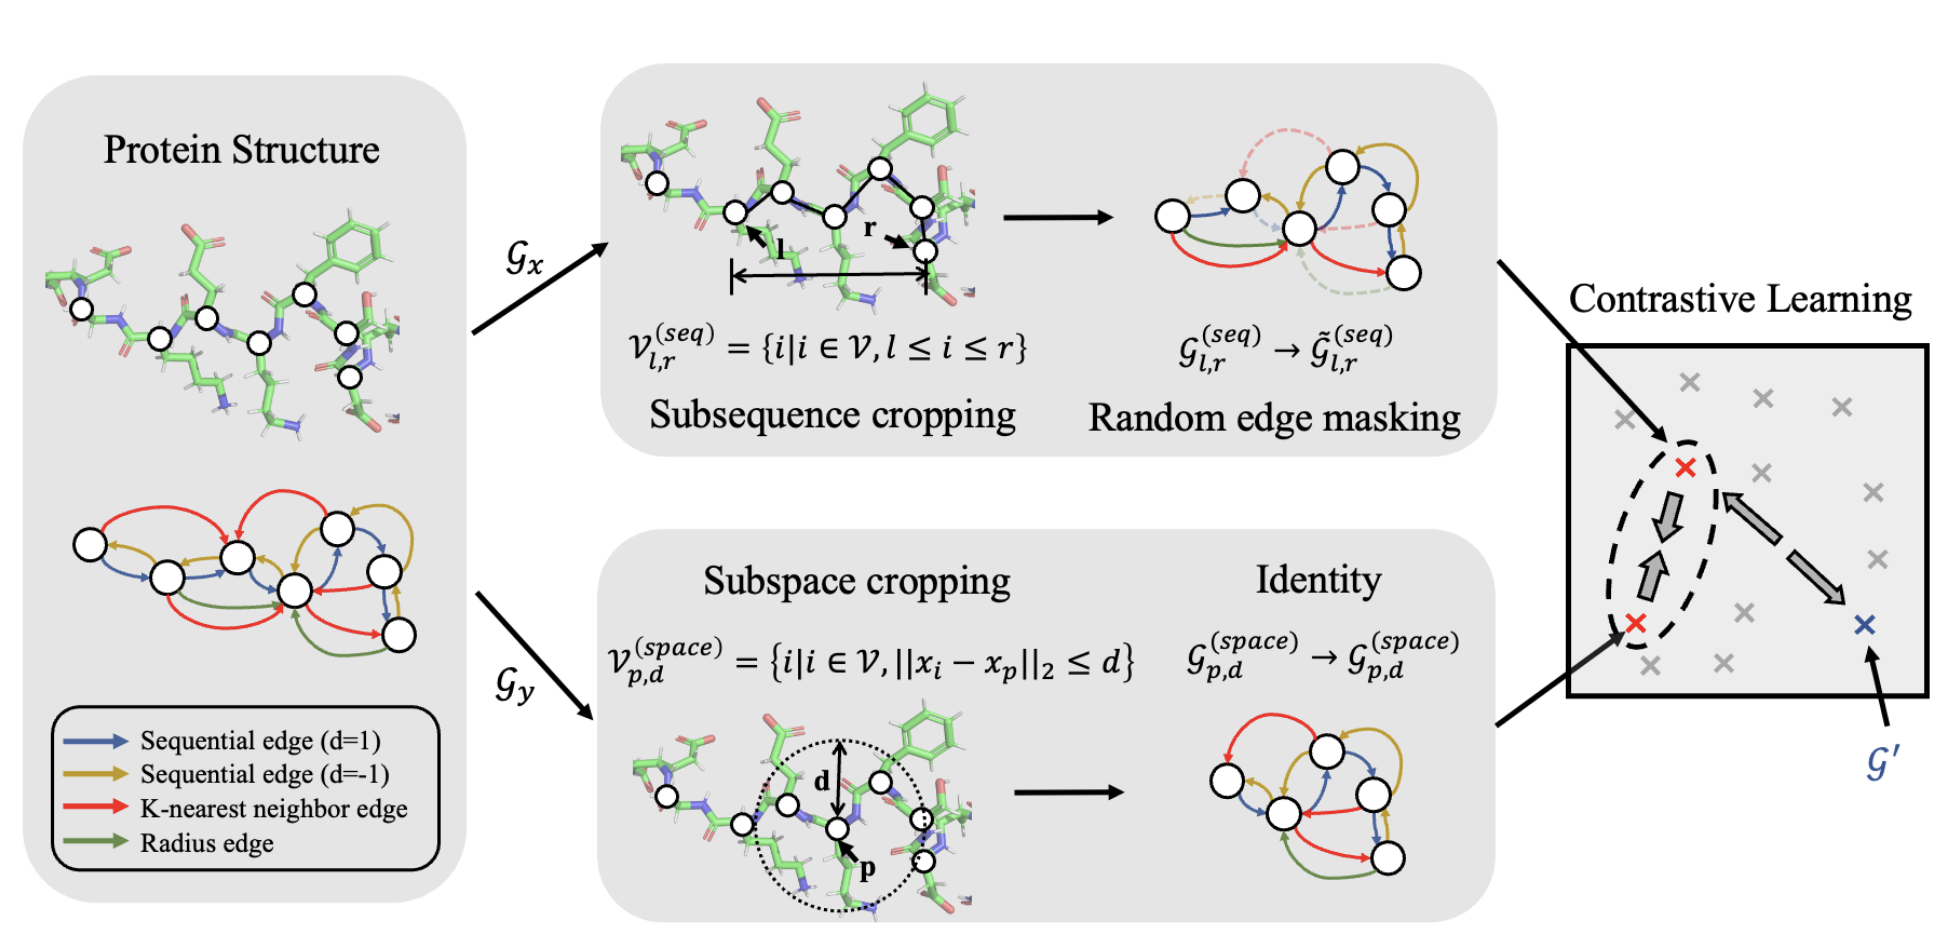
\includegraphics[width=0.95\textwidth]{images/substructure_sampling.png}
\caption{\textbf{Building the positive pair by substructure sampling.} From one
protein's residue graph, two views $\mathcal{G}_x,\mathcal{G}_y$ are drawn by
cropping a connected substructure: either a contiguous chain segment (subsequence,
top) or a spatial ball around a residue (subspace, bottom), optionally followed by
light edge masking. The contrastive loss pulls the two views together in latent
space and pushes other proteins ($\mathcal{G}'$) apart. Adapted from
GearNet~\cite{gearnet}; the substructure-crop idea follows Hermosilla and
Ropinski~\cite{hermosilla}.}
\label{fig:substructure}
\end{figure}

\subsection{The InfoNCE objective}
\label{sec:infonce}

The objective is the NT-Xent form of InfoNCE~\cite{infonce,simclr}, with negatives
taken from the batch. A step samples $M$ proteins and two substructure views of
each, giving $2M$ embeddings $\mathbf{z}_1,\dots,\mathbf{z}_{2M}\in\mathbb{S}^{d_s-1}$
(Section~\ref{sec:readout}); the two views of one protein form a positive pair
$(i,j)$, and the other $2M-2$ views are its negatives. With cosine similarity
$\mathrm{sim}(\mathbf{u},\mathbf{v})=\mathbf{u}^{\top}\mathbf{v}$ and temperature
$\tau$,
\[
\ell_{i,j}=-\log\frac{\exp\!\big(\mathrm{sim}(\mathbf{z}_i,\mathbf{z}_j)/\tau\big)}
{\displaystyle\sum_{a=1}^{2M}\mathbf{1}_{[a\neq i]}\,\exp\!\big(\mathrm{sim}(\mathbf{z}_i,\mathbf{z}_a)/\tau\big)},
\qquad
\mathcal{L}=\frac{1}{2M}\sum_{(i,j)}\ell_{i,j},
\]
the sum running over both ordered directions of every positive pair, with
$\tau=0.2$. The loss acts directly on the sphere embedding $\mathbf{z}$: there is no
projection head and no momentum encoder. A large batch (a single lab GPU allows a
few hundred proteins, i.e.\ several hundred negatives per anchor) supplies enough
negatives for the uniformity term of Section~\ref{sec:training} to spread the
embeddings, so no negative queue is needed.

\section{Plan of experiments}
\label{sec:plan}

\subsection{Metrics}

I evaluate the embeddings by clustering them (HDBSCAN~\cite{hdbscan}, density-based)
and comparing the result to the Foldseek clusters used as reference labels. A
single overlap score such as the adjusted Rand index (ARI) tells me \emph{whether}
the two partitions agree but not \emph{how} they disagree, and the two ways a
clustering can be wrong are opposite and worth separating. I therefore report a
set of directional agreement metrics as the primary readout, and keep ARI and
TM-$\rho$ as secondary summaries.

\paragraph{Notation.} Let $\mathcal{C}=\{C_1,\dots,C_{|\mathcal{C}|}\}$ be the
reference (Foldseek) clusters and $\mathcal{K}=\{K_1,\dots,K_{|\mathcal{K}|}\}$ the
clusters found in the embedding, over $n$ proteins. Write $n_{ck}=|C_c\cap K_k|$ for
the contingency counts, $n_c=|C_c|$, $n_k=|K_k|$, and denote entropies and
conditional entropies by
\[
H(\mathcal{C})=-\sum_c\frac{n_c}{n}\log\frac{n_c}{n},\qquad
H(\mathcal{C}\mid\mathcal{K})=-\sum_k\frac{n_k}{n}\sum_c\frac{n_{ck}}{n_k}\log\frac{n_{ck}}{n_k},
\]
and symmetrically $H(\mathcal{K})$, $H(\mathcal{K}\mid\mathcal{C})$.

\paragraph{Homogeneity, completeness, V-measure.} Following
Rosenberg--Hirschberg~\cite{rosenberg2007},
\[
h=1-\frac{H(\mathcal{C}\mid\mathcal{K})}{H(\mathcal{C})},\qquad
c=1-\frac{H(\mathcal{K}\mid\mathcal{C})}{H(\mathcal{K})},\qquad
V=\frac{2\,h\,c}{h+c}.
\]
Homogeneity $h$ is $1$ when every learned cluster is pure in reference labels
($H(\mathcal{C}\mid\mathcal{K})=0$); completeness $c$ is $1$ when every reference
fold lands in a single learned cluster. They trade off — singletons maximise $h$,
one giant cluster maximises $c$ — and $V$ is their harmonic mean; reporting $h$ and
$c$ separately shows which side is failing.

\begin{figure}[h]
\centering
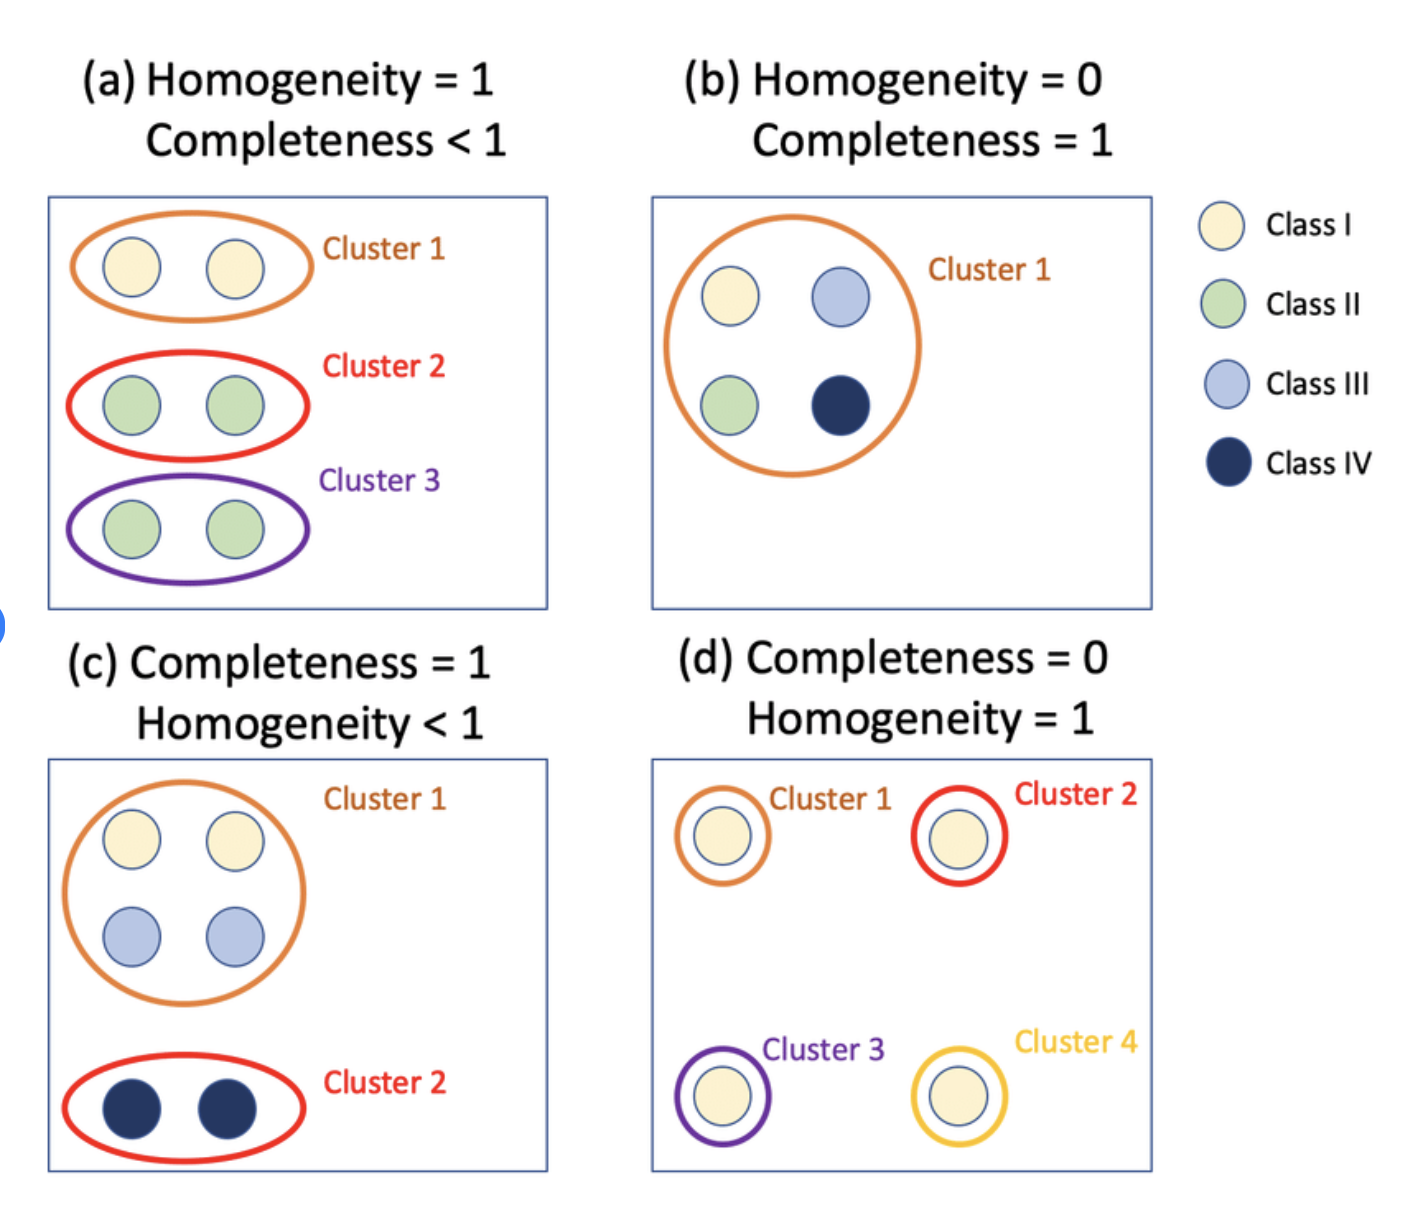
\includegraphics[width=0.72\textwidth]{images/metrics.png}
\caption{\textbf{Homogeneity versus completeness on toy clusterings.} Disc colour is
the ground-truth class (I--IV, key at right); outlines are the predicted clusters.
(a)~clusters are pure but a class is split across several: $h=1$, $c<1$. (b)~a single
cluster mixes every class: $h=0$, $c=1$. (c)~each class stays together but the
clusters are impure: $c=1$, $h<1$. (d)~every protein isolated in its own cluster:
$h=1$, $c=0$. Reporting $h$ and $c$ separately distinguishes over-merging from
over-splitting.}
\label{fig:hc}
\end{figure}

\paragraph{Fragmentation and fusion.} With $\mathcal{K}(C_c)=\{k:n_{ck}>0\}$ the set
of learned clusters a reference fold touches, and $\mathcal{C}(K_k)=\{c:n_{ck}>0\}$
the reference folds a learned cluster touches,
\[
\mathrm{frag}=\frac{1}{|\mathcal{C}|}\sum_{c}\big|\mathcal{K}(C_c)\big|,\qquad
\mathrm{fus}=\frac{1}{|\mathcal{K}|}\sum_{k}\big|\mathcal{C}(K_k)\big|.
\]
Fragmentation is the mean number of learned clusters a fold is split across (the
cluster-level face of low completeness); fusion is the mean number of folds merged
into one learned cluster (the face of low homogeneity); both are $1$ when ideal.
High $\mathrm{frag}$ with low $\mathrm{fus}$ means over-splitting; the reverse means
over-merging.

\begin{figure}[h]
\centering
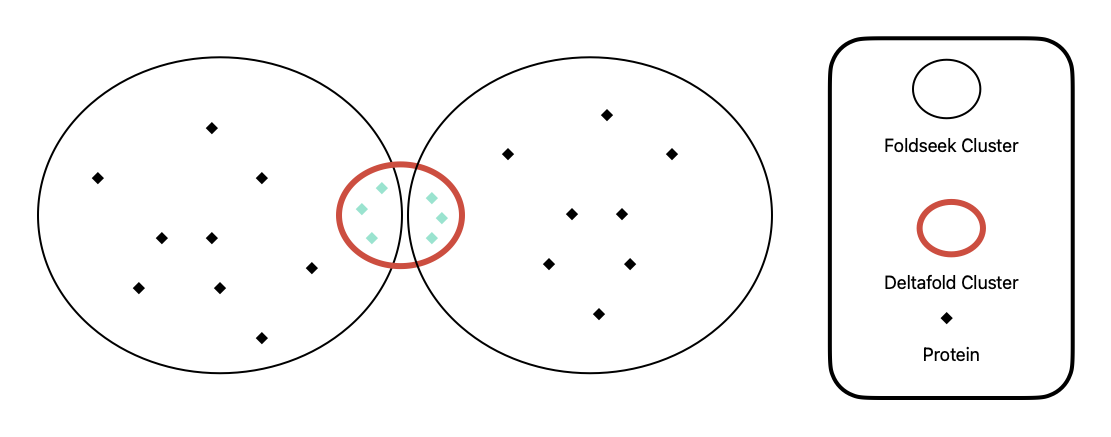
\includegraphics[width=0.78\textwidth]{images/false_positives.png}
\caption{\textbf{False positives at the pair level.} Thin black ellipses are two
distinct Foldseek reference folds; the red ellipse is one DeltaFold cluster that
straddles both. Every pair of the highlighted proteins (green) that it co-clusters
across the two folds is a false positive. The false-positive rate $\mathrm{FPR}$
counts these merged cross-fold pairs over all cross-fold pairs; it is the pair-level
face of fusion (over-merging unrelated folds), the failure mode we most want to
avoid.}
\end{figure}

\paragraph{Pair false-positive and false-negative rates.} At the level of protein
\emph{pairs}, a pair is a positive if the two proteins share a Foldseek reference
fold and a negative otherwise; the learned clustering either co-clusters them or
not. Counting agreements and disagreements over all $\binom{n}{2}$ pairs,
\[
\mathrm{TP}=\sum_{c,k}\binom{n_{ck}}{2},\quad
\mathrm{FP}=\sum_k\binom{n_k}{2}-\mathrm{TP},\quad
\mathrm{FN}=\sum_c\binom{n_c}{2}-\mathrm{TP},\quad
\mathrm{TN}=\binom{n}{2}-\mathrm{TP}-\mathrm{FP}-\mathrm{FN},
\]
where a \emph{false positive} is a pair co-clustered by the model but lying in two
different reference folds (an over-merge), and a \emph{false negative} is a same-fold
pair split apart (an over-split). We report the two rates
\[
\mathrm{FPR}=\frac{\mathrm{FP}}{\mathrm{FP}+\mathrm{TN}}=\frac{\mathrm{FP}}{\binom{n}{2}-\sum_c\binom{n_c}{2}},
\qquad
\mathrm{FNR}=\frac{\mathrm{FN}}{\mathrm{FN}+\mathrm{TP}}=\frac{\mathrm{FN}}{\sum_c\binom{n_c}{2}}.
\]
$\mathrm{FPR}$ is the fraction of cross-fold (negative) pairs the embedding wrongly
glues together --- the pair-level face of fusion --- and $\mathrm{FNR}$ the fraction
of same-fold (positive) pairs it fails to co-cluster --- the pair-level face of
fragmentation. A low $\mathrm{FPR}$ is the primary target, since merging unrelated
folds is the failure mode we most want to avoid; read together, the two rates locate
the model on the over-merge / over-split axis.

\paragraph{TM-$\rho$.} A clustering-free continuous check: over a sampled set
$\mathcal{P}$ of protein pairs with known TM-scores,
\[
\mathrm{TM}\text{-}\rho=\operatorname{Spearman}_{(a,b)\in\mathcal{P}}\big(\,1-\mathbf{z}_a^{\top}\mathbf{z}_b,\ \mathrm{TM}(a,b)\,\big),
\]
the rank correlation between embedding cosine distance and structural similarity.
A negative value is wanted (similar structures close together); it is a secondary
sanity check rather than the primary target.

The practical consequence is that no single epoch is a reliable readout. A fairer
summary is the level and trend of the homogeneity/completeness and
fragmentation/fusion pair over the last several epochs, averaged over a few random
seeds, gated by the health checks of Section~\ref{sec:health}.

\subsection{Baselines}

I want every number reported against two references on the same split: a random
or shuffled-embedding baseline as a floor, and Foldseek~\cite{foldseek} as the
method to beat. A result only means something relative to both.

\subsection{Design variables to sweep}
\label{sec:sweep}

The experiments are organised as one-factor-at-a-time sweeps around a base config,
each run scored on the same cold split (Section~\ref{sec:split}) with the primary
metrics of Section~\ref{sec:plan} (homogeneity/completeness and
fragmentation/fusion) and gated by the health checks of Section~\ref{sec:health}.
The central question is whether the message-passing topology --- in particular the
inter-SSE coupling --- is what limits fold recovery, so the message-passing order is
the first axis.

\paragraph{Message-passing order (tensor diagram).} The main variable. Holding the
model width, depth and objective fixed, we vary the \texttt{-{}-tensor-diagram}
(Section~\ref{sec:modular}):
\begin{itemize}[leftmargin=1.4em,itemsep=1pt]
\item \emph{Topotein default} --- the four-step diagram of Section~\ref{sec:attention}
      (edges with SSE context, SSE update through outer edges, residue refinement,
      protein), the reference.
\item \emph{Residue-hub control} --- SSEs and edges communicate only through rank 0
      (no $N^{2\to1}$), the ablation that isolates the effect of the inter-SSE
      channel.
\item \emph{SSE-adjacency variant} --- add a rank-2 adjacency $A^{2\sim1}$ so SSEs
      exchange messages directly through shared contacts, on top of the outer edges.
\item \emph{Reordered sweeps} --- permute the step order (e.g.\ update residues
      before SSEs, or SSEs before edges) to test the sensitivity to the
      bottom-up-then-down schedule.
\item \emph{No-rank-3 variant} --- drop the protein channel and use a pooling
      readout, testing whether the global cell helps or over-fits.
\end{itemize}
The comparison \emph{Topotein default vs.\ residue-hub control} is the decisive one:
if fragmentation/fusion improve with the outer-edge channel, the earlier
underperformance was topological, not geometric.

\paragraph{Positive-pair construction.} The substructure fraction
$f\in[f_{\mathrm{lo}},f_{\mathrm{hi}}]$ (Section~\ref{sec:substructure}) is the
InfoMin knob and is swept in a small grid, e.g.\ $[0.3,0.5]$, $[0.5,0.8]$,
$[0.7,0.9]$, plus the sampling mode (contiguous chain segment vs.\ spatial ball) and
the minimum substructure size. Too small and the two views stop sharing the fold;
too large and they become near-identical.

\paragraph{Objective and geometry.} Contrastive temperature $\tau\in\{0.05,0.1,0.2\}$;
number of interaction layers $L\in\{3,4,6\}$; vector width $d_v\in\{8,16\}$; TCP
bottleneck $\lambda$; edge-centric vs.\ per-rank frames; and the readout strategy
(node pooling vs.\ protein cell). Each is moved alone from the base config.

\begin{table}[h]\centering\small
\caption{One-factor-at-a-time sweep. Base config in bold; each run changes a single row.}
\begin{tabular}{@{}lll@{}}
\toprule
Axis & Base & Swept values\\
\midrule
Tensor diagram        & \textbf{Topotein 4-step} & residue-hub, $+A^{2\sim1}$, reorderings, no-rank-3\\
Substructure $f$      & \textbf{$[0.5,0.8]$}     & $[0.3,0.5]$, $[0.7,0.9]$\\
Substructure mode     & \textbf{contiguous}      & spatial ball\\
Temperature $\tau$    & \textbf{0.2}             & 0.05, 0.1\\
Layers $L$            & \textbf{4}               & 3, 6\\
Vector width $d_v$    & \textbf{16}              & 8\\
Readout               & \textbf{node pooling}    & protein cell\\
\bottomrule
\end{tabular}
\end{table}

\subsection{Health checks I want to run every epoch}
\label{sec:health}

Because a contrastive encoder can cheat by collapsing all embeddings toward a
common direction, I want to log a few diagnostics every epoch and treat them as
gating criteria rather than something I look at afterwards. These are the spread
of the embedding values per dimension (it should stay clearly above the collapse
threshold of about 0.02), the mean off-diagonal cosine similarity (it should stay
low; values near 0.9 to 0.97 mean the vectors are nearly parallel), and the
effective rank of the embedding covariance as a single number for how many
dimensions are actually being used. I would only interpret a checkpoint
biologically if these are healthy at that epoch.



\section{First results}
\label{sec:results}

This section records the first end-to-end run of the pipeline. It is a
\emph{single configuration and a single seed}, so the numbers are a starting
point rather than a validated result; the aim is to document what was obtained and
to fix the questions that must be answered before any of it is read biologically.

\subsection{The run}

The encoder is the Topotein/TCPNet of Section~\ref{sec:architecture}, trained for
$40$ epochs on a single NVIDIA L40S. Configuration: MoCo contrastive objective with
substructure positives (contiguous, fraction $f\in[0.4,0.7]$), temperature
$\tau=0.2$, queue $K=8192$; residue identity, 3Di and positional encodings all
disabled, so the only per-residue input is the $(\phi,\psi)$ pair and the geometry;
scalar width $d_s=128$, vector width $d_v=16$, $L=4$ interaction layers,
edge-centric chiral frames, node-pooling readout. Train/validation is the cold
Nomburg-cluster split of Section~\ref{sec:split} ($55{,}911$ train / $11{,}787$
validation proteins); reference labels are the Nomburg merged structural clusters
($18{,}192$ clusters). Clustering metrics are HDBSCAN over the $\ell_2$-normalised
validation embeddings versus those reference clusters.

\subsection{Metrics obtained}

The pair and cluster metrics are computed \emph{globally}, over all $\binom{n}{2}$
protein pairs of the full dataset: because HDBSCAN leaves $\approx 53\%$ of proteins as
noise, and a same-fold protein left unclustered is a genuine false negative, each noise
point is treated as its own singleton (an earlier version scored only the ``both
multi-member'' subset, which excluded the noise and singletons and badly under-reported
FNR and fragmentation). HDBSCAN itself has no single density threshold: it extracts a
flat clustering from the whole density hierarchy by cluster persistence, controlled by
\texttt{min\_cluster\_size} and \texttt{min\_samples}. Sweeping those, a central
negative result emerges: \textbf{there is no operating point with both low FNR and
near-zero FPR}. Two ends of the trade-off at epoch~$25$ (full dataset):

\begin{center}
\begin{tabular}{@{}l l l l l@{}}
\toprule
Operating point & FNR & FPR & ARI & noise\\
\midrule
High precision (persistence, $\sim$pure) & $0.90$ & $0.00$ & $0.18$ & $0.53$\\
Higher recall (flat cut $\approx0.25$, \texttt{min\_samples}$=1$) & $0.53$ & $0.15$ & $0.01$ & $0.35$\\
\bottomrule
\end{tabular}
\end{center}

At the precision end the model almost never merges unrelated folds
($\mathrm{FPR}\approx 0$, permutation-null $\mathrm{ARI}\approx 0$) but leaves
$\sim 90\%$ of same-fold pairs unclustered. Pushing for recall (merging more) drops FNR
to $\sim 0.5$ only by raising FPR to $\sim 0.15$ and collapsing ARI toward zero --- the
extra recall comes from indiscriminate merging, not from better structure. In both
regimes the \emph{discrete} agreement with the Nomburg reference is weak, at every
HDBSCAN setting tried.

The \emph{continuous} signal, by contrast, is strong. The clustering-free check is
$\mathrm{TM}\text{-}\rho = -0.69$ over $7{,}059$ sampled pairs: the latent geometry
ranks structural similarity well even though a density clustering of it does not. The
health checks of Section~\ref{sec:health} pass throughout --- per-dimension spread
$\approx 0.075$ (well above the $0.02$ collapse floor), mean off-diagonal cosine
$\approx 0.24$, uniformity $\approx -2.5$, effective rank $\approx 44$ of $128$ --- so
the representation is not collapsed.

The reading so far is therefore mixed: DeltaFold appears to learn a meaningful
\emph{continuous} structural metric (strong TM-$\rho$, healthy geometry), but a
density-based clustering of that space does not reconstruct the Nomburg fold partition.
Whether that is a granularity mismatch (the $18{,}192$ reference clusters being coarser
or finer than the embedding's density structure), folds that are simply not
density-separated, or a genuine limit of the current encoder, is exactly what the
questions below must resolve.

\paragraph{A caveat behind the aggregate.} The largest reference folds are shattered:
the five biggest Nomburg clusters ($1952,1591,1074,855,463$ members) split into
$115,173,95,45$ and $36$ model clusters, $\approx 35$--$53\%$ of each left as noise; and
the \emph{mean} per-cluster FNR across all multi-member reference clusters is
$\approx 0.86$. The favourable-looking numbers of the first draft were an artefact of
the excluded-noise subset, not a property of the model.

\subsection{Questions to confirm a biological signal}
\label{sec:results-questions}

Whether the above is genuine structural learning --- as opposed to an easy shortcut,
a degenerate representation, or an artefact of the reference labels --- is not yet
established. The following must be answered before any biological reading.

\begin{itemize}[leftmargin=1.4em,itemsep=1pt]
\item \emph{Above the floor and below the target?} Report every number against the
      two references of Section~\ref{sec:plan}: a shuffled-embedding baseline and a
      random-initialised encoder (a floor), and Foldseek on the same split (the
      method to beat). Permutation-null ARI $\approx 0$ is necessary but not
      sufficient.
\item \emph{Structural, or a global-shape shortcut?} Sequence and composition
      shortcuts are excluded by construction (no amino-acid, 3Di or positional
      inputs). But the rank-3 cochain carries size, $R_g$ and shape eigenvalues:
      test whether the cluster assignment correlates with chain length / $R_g$, and
      re-measure with the rank-3 channel dropped (the no-rank-3 tensor diagram).
\item \emph{Generalisation, not leakage?} The split is cold at the cluster level, so
      validation folds are unseen; confirm the train--validation gap is small and
      that no reference cluster spans the split.
\item \emph{Is TM-$\rho$ real?} Recompute on a large, uniformly sampled pair set with
      a full TM cache, and check the correlation holds across the whole TM range
      rather than being driven by a few extremes.
\item \emph{Are the mega-fold sub-clusters biology or failure?} For a shattered big
      fold, do the model sub-clusters correspond to meaningful sub-families
      (taxonomy, function, sequence/MSA sub-structure), or are they arbitrary? (This
      is the per-reference-cluster sub-cluster FASTA / alignment analysis.)
\item \emph{Is the reference the right yardstick?} With $18{,}192$ Nomburg clusters,
      fragmentation/fusion partly measure a granularity mismatch; cross-check against
      a second reference (Foldseek at another threshold) and against continuous
      TM-score.
\item \emph{Robustness and the decisive ablation.} Repeat over seeds, and run the
      \emph{Topotein-default vs.\ residue-hub} comparison of Section~\ref{sec:sweep}
      to confirm that the inter-SSE topological channel --- not geometry alone ---
      drives the recovery.
\end{itemize}



\begin{thebibliography}{9}

\bibitem{nomburg2024}
J. Nomburg, E. E. Doherty, N. Price, D. Bellieny-Rabelo, Y. K. Zhu, J. A. Doudna.
\newblock Birth of protein folds and functions in the virome.
\newblock \emph{Nature}, 633:710--717, 2024.
\newblock \url{https://doi.org/10.1038/s41586-024-07809-y}.

\bibitem{topotein}
Z. Wang, A. R. Jamasb, et al.
\newblock Topotein: Topological Deep Learning for Protein Representation Learning.
\newblock \emph{arXiv preprint} arXiv:2509.03885, 2025.

\bibitem{hoan}
M. Hajij, G. Zamzmi, T. Papamarkou, N. Miolane, A. Guzm\'an-S\'aenz,
K. N. Ramamurthy, T. Birdal, T. K. Dey, S. Mukherjee, S. N. Samaga, N. Livesay,
R. Walters, P. Rosen, M. T. Schaub.
\newblock Topological Deep Learning: Going Beyond Graph Data.
\newblock \emph{arXiv preprint} arXiv:2206.00606, 2022.

\bibitem{mpnn}
J. Gilmer, S. S. Schoenholz, P. F. Riley, O. Vinyals, G. E. Dahl.
\newblock Neural Message Passing for Quantum Chemistry.
\newblock \emph{Proceedings of ICML}, 2017. arXiv:1704.01212.

\bibitem{alignunif}
T. Wang, P. Isola.
\newblock Understanding Contrastive Representation Learning through Alignment and
Uniformity on the Hypersphere.
\newblock \emph{Proceedings of ICML}, 2020. arXiv:2005.10242.

\bibitem{simclr}
T. Chen, S. Kornblith, M. Norouzi, G. Hinton.
\newblock A Simple Framework for Contrastive Learning of Visual Representations
(SimCLR).
\newblock \emph{Proceedings of ICML}, 2020. arXiv:2002.05709.

\bibitem{infonce}
A. van den Oord, Y. Li, O. Vinyals.
\newblock Representation Learning with Contrastive Predictive Coding (InfoNCE).
\newblock \emph{arXiv preprint} arXiv:1807.03748, 2018.

\bibitem{foldseek}
M. van Kempen, S. S. Kim, C. Tumescheit, M. Mirdita, J. Lee, C. L. M. Gilchrist,
J. S\"oding, M. Steinegger.
\newblock Fast and accurate protein structure search with Foldseek.
\newblock \emph{Nature Biotechnology}, 42:243--246, 2024.

\bibitem{hdbscan}
R. J. G. B. Campello, D. Moulavi, J. Sander.
\newblock Density-Based Clustering Based on Hierarchical Density Estimates
(HDBSCAN).
\newblock \emph{Advances in Knowledge Discovery and Data Mining (PAKDD)}, 2013.

\bibitem{gvp}
B. Jing, S. Eismann, P. Suriana, R. J. L. Townshend, R. Dror.
\newblock Learning from Protein Structure with Geometric Vector Perceptrons.
\newblock \emph{Proceedings of ICLR}, 2021. arXiv:2009.01411.

\bibitem{gcpnet}
A. Morehead, J. Cheng.
\newblock Geometry-Complete Perceptron Networks for 3D Molecular Graphs.
\newblock \emph{Bioinformatics}, 2024. arXiv:2211.02504.

\bibitem{bro2008}
R. Bro, E. Acar, T. G. Kolda.
\newblock Resolving the Sign Ambiguity in the Singular Value Decomposition.
\newblock \emph{Journal of Chemometrics}, 22:135--140, 2008.

\bibitem{rbf}
K. T. Sch\"utt, P.-J. Kindermans, H. E. Sauceda, S. Chmiela, A. Tkatchenko,
K.-R. M\"uller.
\newblock SchNet: A Continuous-Filter Convolutional Neural Network for Modeling
Quantum Interactions.
\newblock \emph{Advances in Neural Information Processing Systems (NeurIPS)}, 2017.
arXiv:1706.08566.

\bibitem{moco}
K. He, H. Fan, Y. Wu, S. Xie, R. Girshick.
\newblock Momentum Contrast for Unsupervised Visual Representation Learning (MoCo).
\newblock \emph{Proceedings of CVPR}, 2020. arXiv:1911.05722.

\bibitem{hermosilla}
P. Hermosilla, T. Ropinski.
\newblock Contrastive Representation Learning for 3D Protein Structures.
\newblock \emph{arXiv preprint} arXiv:2205.15675, 2022.

\bibitem{gearnet}
Z. Zhang, M. Xu, A. Jamasb, V. Chenthamarakshan, A. Lozano, P. Das, J. Tang.
\newblock Protein Representation Learning by Geometric Structure Pretraining
(GearNet).
\newblock \emph{Proceedings of ICLR}, 2023. arXiv:2203.06125.

\bibitem{dimcol}
L. Jing, P. Vincent, Y. LeCun, Y. Tian.
\newblock Understanding Dimensional Collapse in Contrastive Self-Supervised
Learning.
\newblock \emph{Proceedings of ICLR}, 2022. arXiv:2110.09348.

\bibitem{rosenberg2007}
A. Rosenberg, J. Hirschberg.
\newblock V-Measure: A Conditional Entropy-Based External Cluster Evaluation
Measure.
\newblock \emph{Proceedings of EMNLP-CoNLL}, 2007.

\end{thebibliography}

\end{document}
